\section*{CHƯƠNG 1.  KIẾN THỨC CHUẨN BỊ}
\phantomsection\addcontentsline{toc}{section}{\numberline{}\hspace{-1cm}CHƯƠNG 1.  KIẾN THỨC CHUẨN BỊ}
\setcounter{section}{1}
\setcounter{figure}{0}
\setcounter{table}{0}
\subsection{Phương trình vi phân tuyến tính và bài toán giá trị ban đầu}
Rất nhiều bài toán trong sinh học, khoa học kỹ thuật và công nghiệp gắn liền với việc giải một phương trình vi phân, tức là một phương trình thể hện mối liên hệ của một hàm số chưa biết (cần tìm) với các đạo hàm của nó, xem \cite{ref1}, \cite{ref4}, \cite{ref6}. Luận văn này tập trung vào việc phân tích và mô phỏng (sử dụng phầm mềm Excel, xem \cite{ref2}, \cite{ref5}) các phương trình vi phân tuyến tính bậc nhất có dạng                                
\begin{equation}
	A(t)y'(t)+B(t)y=C(t),
	\label{eq:1.1}
\end{equation}
với mọi $  t \in [{t}_{0},{{t}_{f}})$       \\
trong đó $t$ là biến thời gian, $y(t)$ là hàm chưa biết, $A(t)$, $B(t)$, $C(t)$ là các hàm số nhận giá trị thực cho trước và liên tục trong khoảng    $[t_0, t_f)$        đang xét. \\
Nếu trong khoảng đang xét mà $A(t)\ne 0\,\,\forall t$ thì bằng cách chia cho $A(t)$, phương trình trên có thể đưa được về dạng         
\begin{equation}
	y'(t)+P(t)y=Q(t).
	\label{eq:1.2}
\end{equation}
Cùng với (\ref{eq:1.2}), ta cũng xét phương trình tuyến tính thuần nhất tương ứng có dạng 
\begin{equation}
	y'(t)+P(t)y=0.
	\label{eq:1.3}
\end{equation}
Các phương trình (\ref{eq:1.2}) và (\ref{eq:1.3}) đều có vô số nghiệm. Thông thường thì các phương trình đó cần được ghép cặp với một thông tin bổ sung (điều kiện ban đầu, điều kiện biên) để dẫn đến sự tồn tại duy nhất nghiệm.  Trong nhiều ứng dụng, người ta quan tâm đến bài toán giá trị ban đầu  
\begin{equation}
	\left\{ \begin{array}{l}
	y'(t)+P(t)y=Q(t) \\ 
	y({{t}_{0}})=\,{{y}_{0}} \\ 
\end{array} \right.
\label{eq:1.4}
\end{equation}
trong đó phương trình thứ hai được gọi là điều kiện ban đầu. \\
Bài toán giá trị ban đầu (\ref{eq:1.4}) có công thức nghiệm tường minh, còn được gọi là công thức biến thiên hằng số (variational of constant). Để đảm bảo cho tính toàn vẹn của luận văn, và phù hợp với học sinh phổ thông, cách xây dựng các công thức này sẽ được trình bày lại chi tiết như sau đây. \\
\underline{Bước 1:} Xét phương trình tuyến tính thuần nhất (\ref{eq:1.3}). Giả sử $y\ne 0$  khi đó phương trình  (\ref{eq:1.3}) đưa được về dạng $$\frac{y'(t)}{y(t)}  =-\,P(t).$$
Do đó lấy tích phân hai vế từ ${{t}_{0}}$ đến $t$ ta được 
\[\ln\left| y(t) \right|=-\,\,\int\limits_{{{t}_{0}}}^{t}{P(s)ds\,+\,\ln |{{C}_{1}}|\,\,\,\,\,\,\,\,\,\,\,\,\,\,\,\,\,\,({{C}_{1}}=y({{t}_{o}})\ne 0).}\]
Vì vậy ta có                           
\begin{equation}
	y(t)\,=\,\,y({{t}_{0}})\,{{e}^{-\int\limits_{{{t}_{0}}}^{t}{P(s)ds}}}\,\,\,\,\,.  
	\label{eq:1.5}
\end{equation}                                   Trong trường hợp điều kiện ban đầu chưa biết, ta có thể xét công thức nghiệm của phương trình (\ref{eq:1.3}) dưới dạng 
\begin{equation}
	y(t)\,=\,\,C\,{{e}^{-\int\limits_{{{t}_{0}}}^{t}{P(s)ds}}}.
\label{eq:1.6}
\end{equation}
\underline{Bước 2:} Trong bước này ta đi tìm nghiệm của (\ref{eq:1.2}) có dạng tương tự (\ref{eq:1.6}), tuy nhiên ở đây thay vì hằng số $C$ ta sẽ xét hàm $C(t)$. \\
Khi đó ta có
\begin{equation}
	y(t)\,=\,\,C(t)\,\,{{e}^{-\int\limits_{{{t}_{0}}}^{t}{P(s)ds}}}.
	\label{eq:1.7}
\end{equation}
Hiển nhiên $y({{t}_{0}})=C({{t}_{0}})$ và \[\frac{dy}{dt}=\dfrac{dC}{dt}\,{{e}^{-\int\limits_{_{{{t}_{0}}}}^{t}{P(s)ds}}}-P(t)\,C\,{{e}^{-\int\limits_{_{{{t}_{0}}}}^{t}{P(s)ds}}}\,.\]
Thay hệ thức này vào phương trình (\ref{eq:1.2}) ta có \[\dfrac{dC}{dt}\,{{e}^{-\int\limits_{_{{{t}_{0}}}}^{t}{P(s)ds}}}-P(t)\,C\,{{e}^{-\int\limits_{_{{{t}_{0}}}}^{t}{P(s)ds}}}\,\,+P(t)\,\,C\,{{e}^{-\int\limits_{_{{{t}_{0}}}}^{t}{P(s)ds}}}\,\,=\,\,Q(t)\,.\]
Do đó $\dfrac{dC}{dt}\,{{e}^{-\int\limits_{_{{{t}_{0}}}}^{t}{P(s)ds}}}\,=\,\,Q(t)\,$. Điều này dẫn đến \[C'(t)\,\,=\,\,{{e}^{\int\limits_{{{t}_{0}}}^{t}{P(s)ds}}}Q(t).\]
Vì $C({{t}_{0}})\,\,=\,y({{t}_{0}})\,$ nên ta có thể lấy tích phân từ ${{t}_{o}}$ đến $t$ để thu được \[C(t)\,=\,\,C({{t}_{0}})\,\,+\,\,\,\int\limits_{{{t}_{0}}}^{t}{{{e}^{\int\limits_{{{t}_{0}}}^{s}{P(z)dz}}}}\,\,Q(s)\,ds\,\,=\,\,\,\,C({{t}_{0}})\,\,+\,{{e}^{\int\limits_{{{t}_{0}}}^{t}{P(z)dz}}}\,\,\,\int\limits_{{{t}_{0}}}^{t}{{{e}^{-\int\limits_{s}^{t}{P(z)dz}}}}\,\,Q(s)\,ds\,.\]
Thay $C(t)$ vào công thức (\ref{eq:1.7}) và chú ý rằng $y({{t}_{0}})=C({{t}_{0}})$ ta thu được 
\begin{equation}
	y(t)\,=\,\,y({{t}_{0}})\,\,{{e}^{-\int\limits_{{{t}_{0}}}^{t}{P(s)ds}}}\,+\,\,\,\int\limits_{{{t}_{0}}}^{t}{{{e}^{-\int\limits_{s}^{t}{P(z)dz}}}}\,\,Q(s)\,ds.
	\label{eq:1.8}
\end{equation}
\textbf{Ví dụ 1.1.} Tìm công thức nghiệm tường minh cho bài toán giá trị ban đầu
\[\left\{ \begin{array}{l}
	 y'(t)-\dfrac{y}{t}={{t}^{2}}\,\,\,\forall \,t>\,1,\, \\ 
	 y(1)\,=\,{{y}_{0}}. \\ 
\end{array} \right.\]
\textbf{Lời giải.}\\
Áp dụng công thức (\ref{eq:1.8}) với $P\left( t \right)=-\dfrac{1}{t},\,\,Q(t)={{t}^{2}}$ ta có \[y(t)\,=\,\,y(1)\,\,{{e}^{\int\limits_{1}^{t}{\frac{1}{s}ds}}}\,+\,\,\,\int\limits_{1}^{t}{{{e}^{\int\limits_{s}^{t}{\frac{1}{z}dz}}}}\,\,{{s}^{2}}\,ds\,\,=\,\left( {{y}_{0}}-\dfrac{1}{2} \right)\,t\,+\,\dfrac{{{t}^{3}}}{2}.\]
Vậy nghiệm của phương trình là $y(t)=\dfrac{{{t}^{3}}}{2}+\left( {{y}_{0}}-\dfrac{1}{2} \right)\,t\,.$\\
\textbf{Chú ý 1.1.
} Trong một số bài toán, khi ta chưa được cho trước điều kiện ban đầu thì thay vì công thức (\ref{eq:1.8}) ta sẽ sử dụng công thức dựa trên nguyên hàm thay vì tích phân như sau
\begin{equation}
	y(t)\,=\,\,C\,{{e}^{-\int{P(t)dt}}}\,+\,{{e}^{-\int{P(t)dt}}}\,\int{{{e}^{\int{P(t)dt}}}}\,Q(t)\,dt.
\label{eq:1.9}
\end{equation}
\subsection{Giải gần đúng bài toán giá trị ban đầu bằng phương pháp Euler tiến}
Xét bài toán giá trị ban đầu (\ref{eq:1.4}), ta thấy rằng có công thức nghiệm tường minh (\ref{eq:1.8}). Tuy vậy, việc tính toán chính xác tích phân  $\int\limits_{_{{{t}_{0}}}}^{t}{P(s)ds}\,$ không phải luôn luôn thực hiện được. Mặt khác, trong nhiều bài toán ứng dụng trong thực tiễn, ta chỉ cần tính xấp xỉ nghiệm đến một mức độ chính xác nhất định. Chính vì vậy các phương pháp số được xây dựng để xấp xỉ nghiệm của bài toán (\ref{eq:1.4}). Để phù hợp với trình độ của học sinh phổ thông trung học, luận văn này chỉ xét phương pháp Euler tiến. Đây là một phương pháp cơ bản và tương đối đơn giản nhưng vẫn thường được sử dụng, xem~ \cite{ref2}.\\
Cơ sở của phương pháp Euler tiến dựa trên việc xấp xỉ đạo hàm bởi sai phân $$y'(t)\approx \dfrac{y(t+h)-y(t)}{h}.$$
trong đó $h$ là một số thực dương đủ nhỏ. Để giải bài toán giá trị ban đầu (\ref{eq:1.4}), ta chia nhỏ đoạn $\,\!\![{{t}_{0}},{{t}_{f}})$ thành N đoạn nhỏ bằng nhau, mỗi đoạn có độ dài $h$ (được gọi là bước). Đặt $\,\,\,{{t}_{n}}={{t}_{0}}+nh$, với $n=0, 1, 2, 3...$ Khi đó ta có
$$\dfrac{y({{t}_{n+1}})-y({{t}_{n}})}{h}\,\approx \,y'({{t}_{n}})=\,-P({{t}_{n}})\,y({{t}_{n}})\,+\,Q({{t}_{n}})\,\,.$$
Do đó ta có $y({{t}_{n+1}})\,\,\approx \,\,(1-hP({{t}_{n}})\,)\,y({{t}_{n}})\,\,+\,\,h\,Q({{t}_{n}})\,$.\\
Ta đặt giá trị xấp xỉ của nghiệm tại thời điểm ${{t}_{n}}$ là ${{y}_{n}}\,\approx y({{t}_{n}})$ khi đó ta có thể tính lần lượt   ${{y}_{n}}\,,\,n\,\,=\,0,\,1,2,....\,$ sử dụng công thức Euler tiến 
\begin{equation}
	{{y}_{n+1}}\,\,\approx \,\,(1-h\,P({{t}_{n}})\,)\,{{y}_{n}}\,\,+\,\,h\,Q({{t}_{n}}).
\label{eq:1.10}
\end{equation}
Trong ví dụ minh họa dưới đây, ta sẽ thấy rằng phương pháp Euler là tương đối chính xác nếu như bước $h$ là đủ nhỏ. Giá trị bước $h$ càng nhỏ thì sai số càng thấp.\\
\textbf{Ví dụ 1.2.} Xét bài toán giá trị ban đầu được đề cập trong Ví dụ 1.1.
\begin{equation}
	\left\{ \begin{array}{l}
	 y'(t)-\dfrac{y}{t}={{t}^{2}},\,\,\forall \,t>\,1,\, \\ 
	 y(1)\,\,=\,\,\dfrac{3}{2}. \\ 
\end{array} \right.
\label{eq:1.11}
\end{equation}
Theo Ví dụ 1.1. ta thấy rằng nghiệm chính xác của bài toán (\ref{eq:1.11}) là $y(t)=~\dfrac{{{t}^{3}}}{2}+~t\,.$\\
Giả sử rằng ta muốn tìm nghiệm xấp xỉ của bài toán (\ref{eq:1.11}) trên đoạn $[1,3]$, chính xác đến $4$ chữ số thập phân bằng cách sử dụng phương pháp Euler tiến. \\
Ta chia đoạn $[1,3]$ thành N đoạn nhỏ có độ dài $h$ và đặt ${{t}_{n}}:=1\,+n\,h$, ${{y}_{n}}:=y({{t}_{n}}).$ \\
Khi đó ta có thể tính lần lượt các giá trị xấp xỉ  ${{y}_{n}}\,$với $n=0,1,2,...$ sử dụng công thức
\[{{y}_{n+1}}\,\,\approx \,\,(1+\dfrac{h}{{{t}_{n}}}\,)\,{{y}_{n}}\,\,+\,\,h\,\,t_{n}^{2}.\]
Tại mỗi thời điểm ${{t}_{n}}$ ta xác định các công thức sai số như sau\\ 
Sai số tuyệt đối  tại thời điểm ${{t}_{n}}$ là  $$\Delta {{y}_{n}}:=\left| y({{t}_{n}})-{{y}_{n}} \right|\,$$ 
Sai số tương đối  tại thời điểm ${{t}_{n}}$ là \\ $$\delta {{y}_{n}}:=\dfrac{\left| y({{t}_{n}})-{{y}_{n}} \right|\,}{\left| y({{t}_{n}}) \right|}\,\,\times \,\,100\%=\dfrac{\Delta {{y}_{n}}}{\left| y({{t}_{n}}) \right|}\times \,\,100\% $$\\
Trong khi sai số tuyệt đối xác định sai số so với nghiệm chính xác thì sai số tương đối cho thấy mức độ sai số tính theo phần trăm. Sai số tương đối phù hợp hơn sai số tuyệt đối trong những bài toán mà nghiệm chính xác quá lớn hoặc quá nhỏ, xem [2,4]. Sau đây ta đi thực hiện quá trình xấp xỉ nghiệm trên trong Excel.\newpage
\noindent \underline{Bước 1:} Nhập các tham số sử dụng trong công thức $(h, n, y(1)).$
\begin{center}
	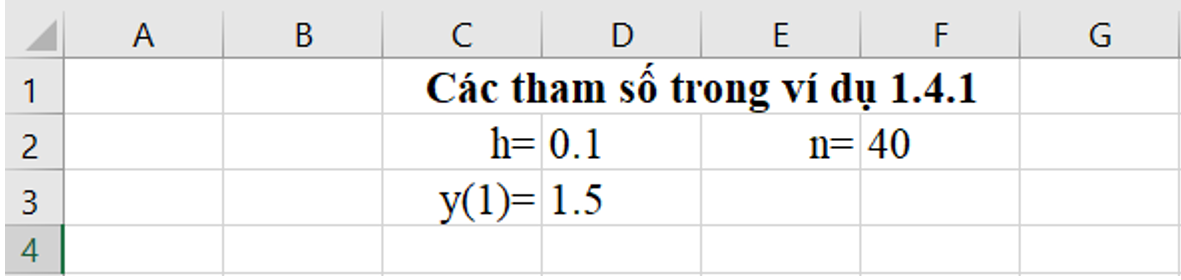
\includegraphics[scale=0.6]{Images/cac_tham_so_trong_vidu_1_4_1}
\end{center}
\underline{Bước 2:} Lập bảng gồm các cột: $n$, ${{t}_{n}}$, nghiệm xấp xỉ, nghiệm chính xác, sai số tuyệt đối, sai số tương đối (\%). \\
\underline{Bước 3.} Tính giá trị ở các cột.\\
+ Cột n: nhận các giá trị từ $0$ đến $40$.\\
+ Cột ${{t}_{n}}$ được tính bằng công thức ${{t}_{n}}:=1\,+n\,h$
\begin{center}
	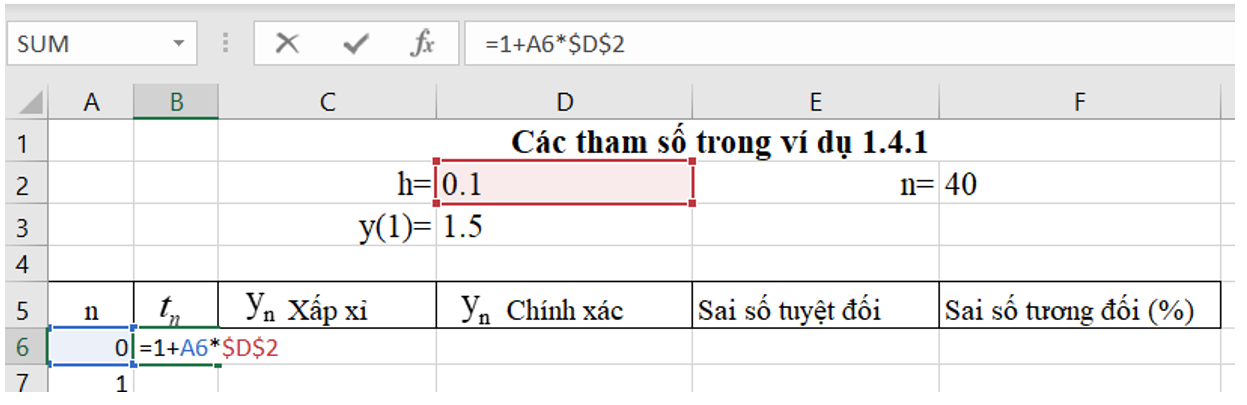
\includegraphics[scale=0.7]{Images/cac_tham_so_trong_vidu_1_4_1t}
\end{center}
+ Cột ${{y}_{n}}$ xấp xỉ được tính bằng công thức ${{y}_{n+1}}\,\,\approx \,\,(1+\dfrac{h}{{{t}_{n}}}\,)\,{{y}_{n}}\,\,+\,\,h\,\,t_{n}^{2}.$
\begin{center}
	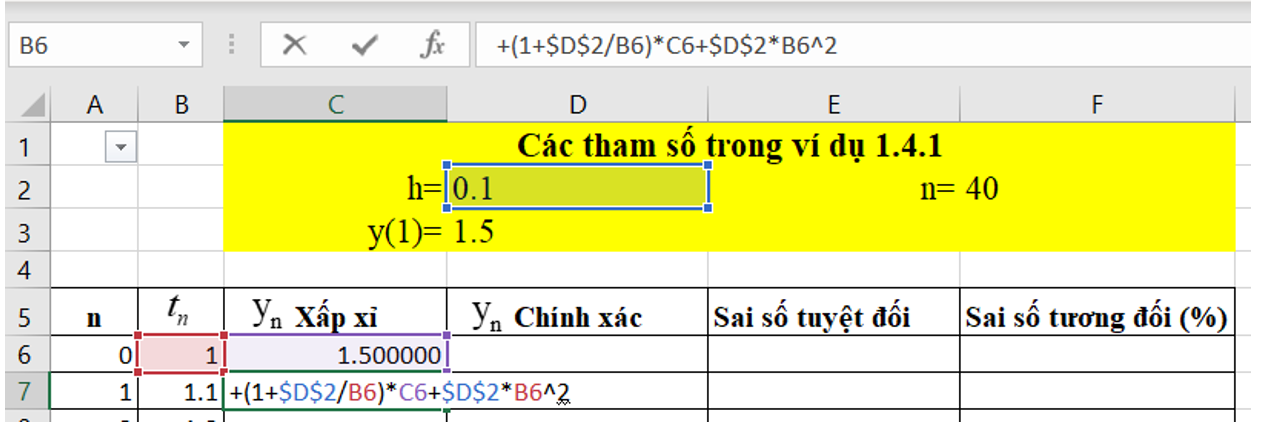
\includegraphics[scale=0.7]{Images/cac_tham_so_trong_vidu_1_4_1tt}
\end{center}\newpage
+ Cột ${{y}_{n}}$ chính xác được tính bằng công thức $y(t)=\dfrac{{{t}^{3}}}{2}+t\,.$
\begin{center}
	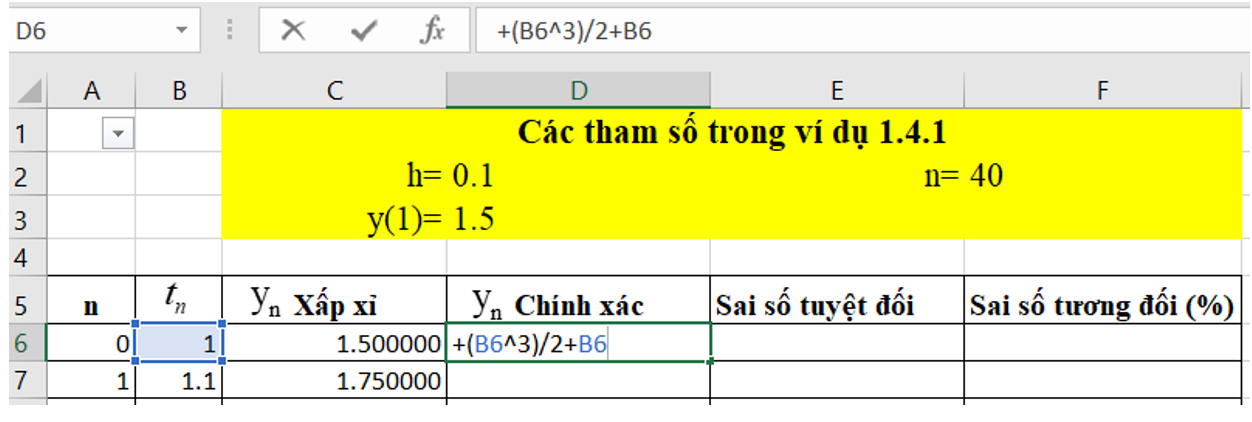
\includegraphics[scale=0.7]{Images/cac_tham_so_trong_vidu_1_4_1ttt}
\end{center}
+ Sai số tuyệt đối được tính bằng công thức  $\left|y_n\right.$ chính xác $-$ $y_n$ xấp xỉ $\left.\right|$
\begin{center}
	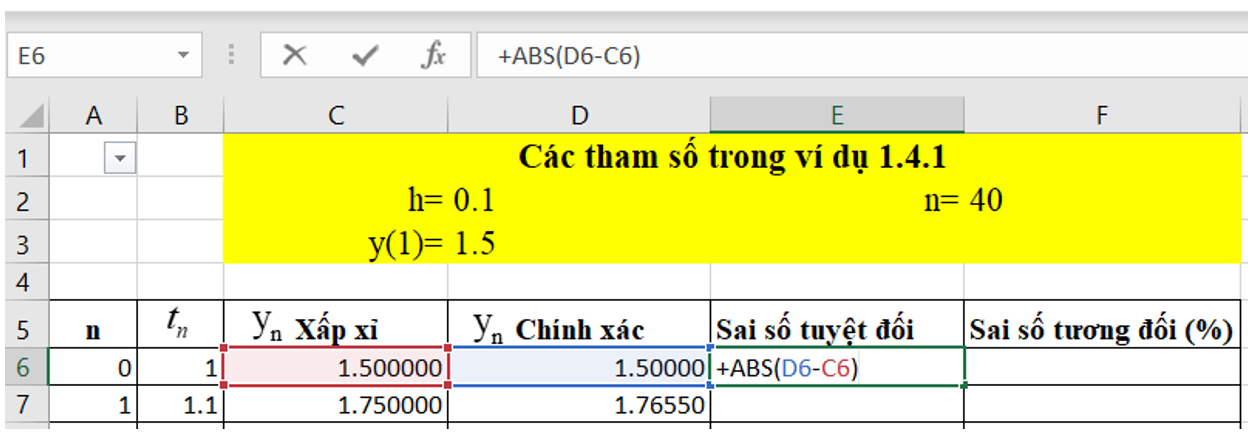
\includegraphics[scale=0.7]{Images/cac_tham_so_trong_vidu_1_4_1tttt}
\end{center}
	+ Sai số tương đối (\%) được tính bằng công thức
\begin{center}
	(Sai số tuyệt đối : ${{y}_{n}}$ chính xác) x 100
\end{center}
\begin{center}
	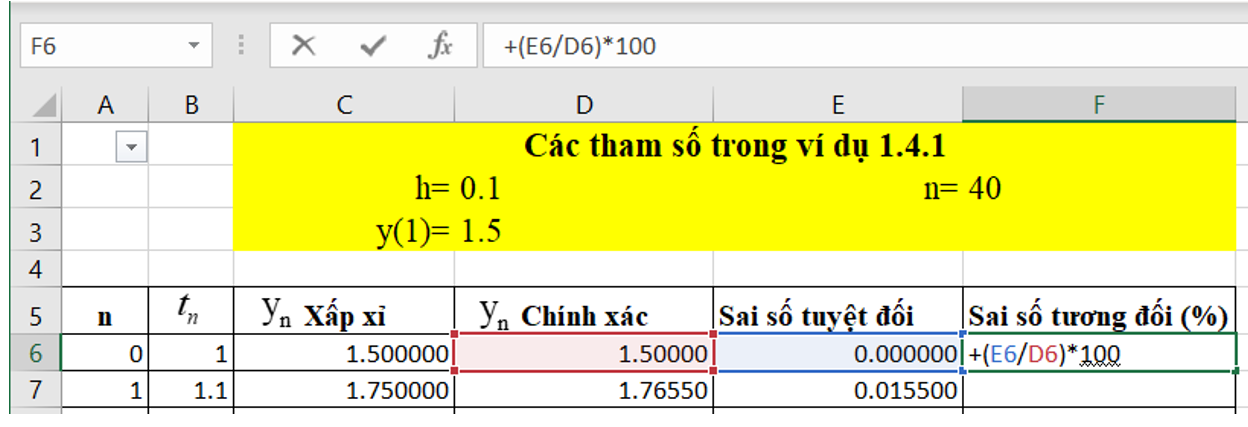
\includegraphics[scale=0.7]{Images/cac_tham_so_trong_vidu_1_4_1t5}
\end{center}
\underline{Bước 4.} Vẽ đồ thị\\
+ Ta trích xuất $1$ bảng gồm các giá trị tương ứng với số thứ tự $n$ chia hết cho $5$ (ta sử dụng filter để lọc dữ liệu) 
\begin{center}
	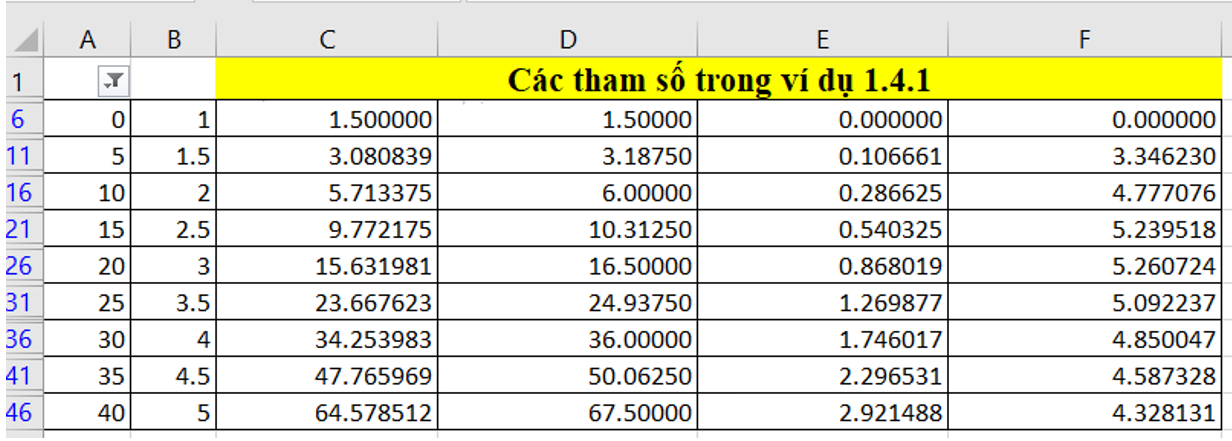
\includegraphics[scale=0.7]{Images/cac_tham_so_trong_vidu_1_4_1t6}
\end{center}
+ Từ bảng trích xuất ta vẽ đồ thị nghiệm xấp xỉ: \\
Chọn $2$ cột ${{t}_{n}}$ và nghiệm xấp xỉ $\rightarrow$  chọn insert $\rightarrow$ chọn insert line or Area chart \newline$\rightarrow$ chọn vào dạng đồ thị phù hợp
\begin{center}
	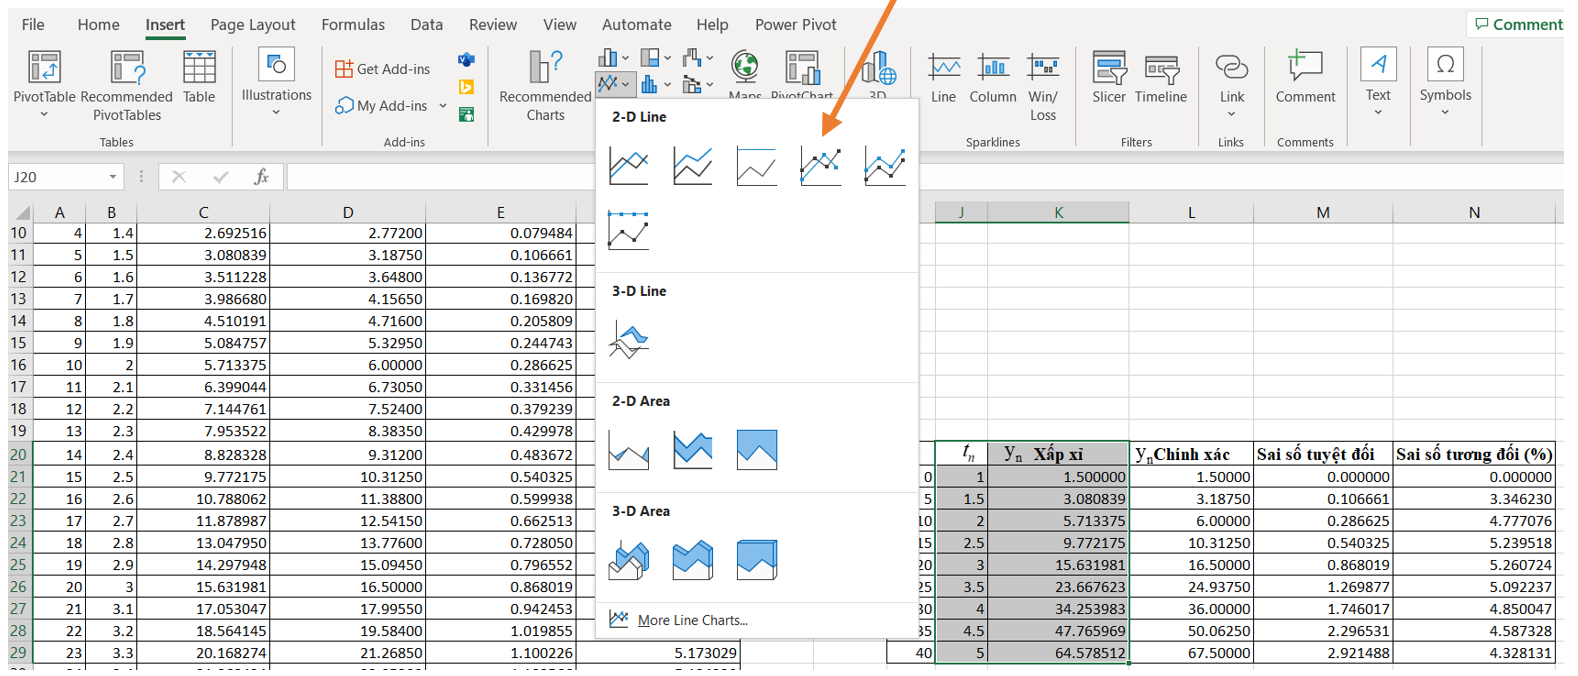
\includegraphics[scale=0.57]{Images/cac_tham_so_trong_vidu_1_4_1t7}
\end{center}
+ Để vẽ đồ thị sai số tuyệt đối và sai số tương đối của nghiệm xấp xỉ:\\
Chọn $2$ cột sai số tuyệt đối và sai số tương đối $\rightarrow$ chọn insert $\rightarrow$ chọn insert line or Area chart $\rightarrow$ chọn vào dạng đồ thị phù hợp
\begin{center}
	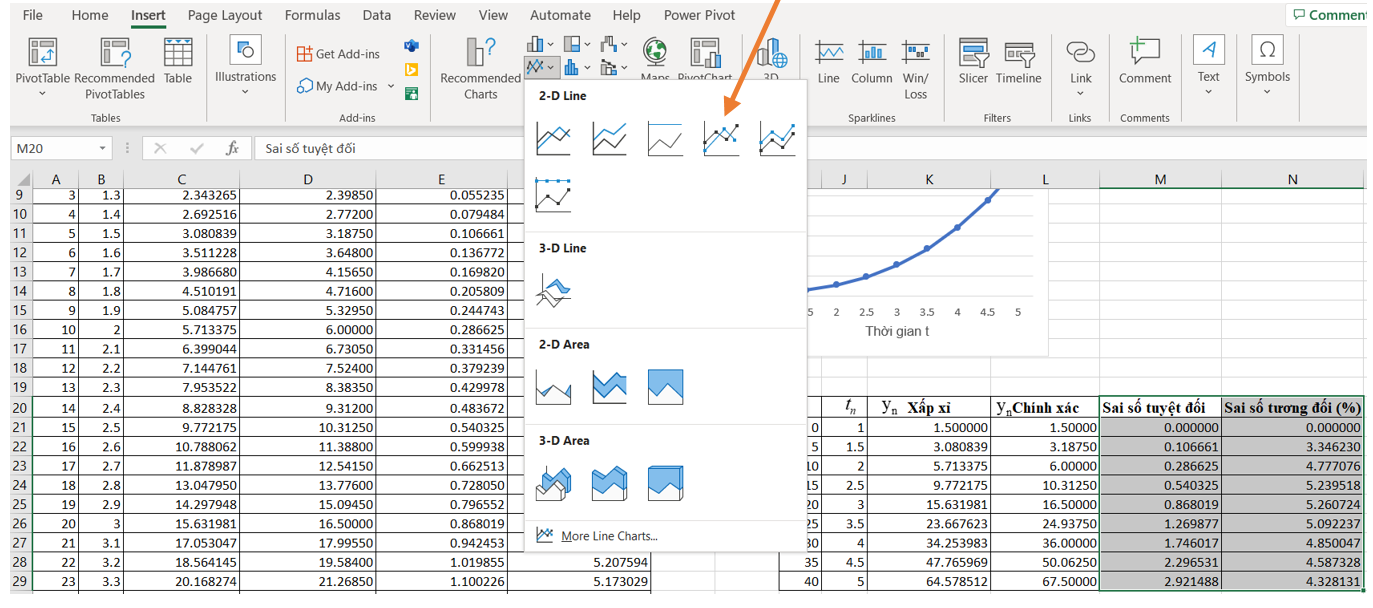
\includegraphics[scale=0.65]{Images/cac_tham_so_trong_vidu_1_4_1t8}
\end{center}
Xét trường hợp $h = 0.1$, trong bảng dưới đây ta giải số nghiệm của (\ref{eq:1.11}) cùng với sai số tuyệt đối và sai số tương đối tại mỗi giá trị ${{t}_{n}}\,$.
\begin{table}[H]
	\centering
	\begin{tabularx}{\textwidth}{
			|>{\centering\arraybackslash}s
			|>{\centering\arraybackslash}s
			|>{\centering\arraybackslash}y
			|>{\centering\arraybackslash}y
			|>{\centering\arraybackslash}y
			|>{\centering\arraybackslash}y|
		}
		\hline
		\bfseries  n  
		&\bfseries  $\mathbf{t}_{\mathbf{n}}$
		& \bfseries Nghiệm 
		xấp xỉ
		& \bfseries Nghiệm 
		chính xác
		& \bfseries Sai số 
		tuyệt đối
		& \bfseries Sai số 
		tương đối (\%)
		\\
		\hline
		0 &	1	 &   1.5000	&   1.5000  & 0.0000 &	0.0000 \\ \hline
		1 &	1.1	 &   1.7500 &  	1.7655  & 0.0155 &	0.8779 \\ \hline
		2 &	1.2	 &   2.0301 &	2.0640  & 0.0339 &	1.6429 \\ \hline
		3 &	1.3	 &   2.3433	&   2.3985  & 0.0552 &	2.3029 \\ \hline
		4 &	1.4	 &   2.6925	&   2.7720  & 0.0795 &	2.8674 \\ \hline
		5 &	1.5	 &   3.0808	&   3.1875  & 0.1067 &	3.3462 \\ \hline
		6 &	1.6	 &   3.5112	&   3.6480  & 0.1368 &	3.7492 \\ \hline
		7 &	1.7	 &   3.9867	&   4.1565  & 0.1698 &	4.0857 \\ \hline
		8 &	1.8	 &   4.5102	&   4.7160  & 0.2058 &	4.3641 \\ \hline
		9 &	1.9	 &   5.0848	&   5.3295  & 0.2447 &	4.5922 \\ \hline
		10 & 2	 &   5.7134	&   6.0000  & 0.2866 &	4.7771 \\ \hline
		11 & 2.1 &	 6.3990	&   6.7305  & 0.3315 &	4.9247 \\ \hline
		12 & 2.2 &	 7.1448	&   7.5240  & 0.3792 &	5.0404 \\ \hline
		13 & 2.3 &	 7.9535	&   8.3835  & 0.4300 &	5.1289 \\ \hline
		14 & 2.4 &	 8.8283	&   9.3120  & 0.4837 &	5.1941 \\ \hline
		15 & 2.5 &	 9.7722	&   10.3125 & 0.5403 &	5.2395 \\ \hline
		
		
	\end{tabularx}
	\caption[Bảng số liệu giá trị nghiệm bằng phương pháp Euler tiến với $h = 0.1.$]{\itshape\fontsize{13pt}{0pt}\selectfont Bảng số liệu giá trị nghiệm bằng phương pháp Euler tiến với $h = 0.1.$}
	\label{bang1}
\end{table}
\begin{figure}[H]
	\centering
	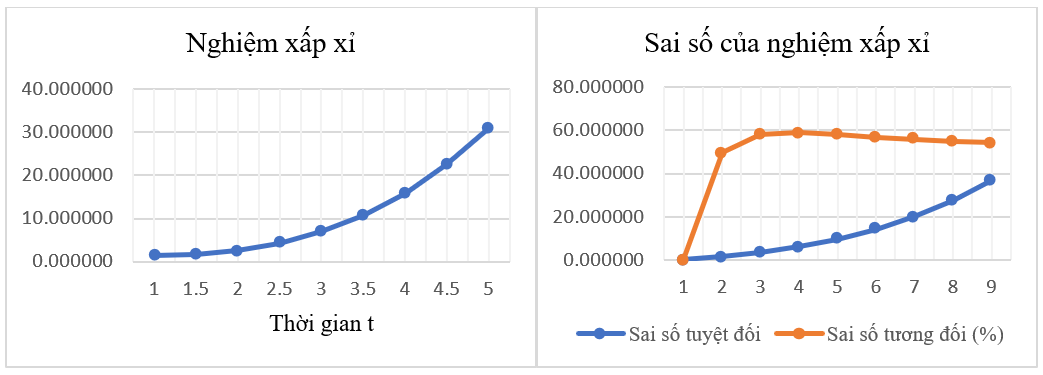
\includegraphics[scale=0.7]{Images/hinh_1_1.png}
	\caption[Biểu đồ nghiệm xấp xỉ và sai số với bước $h = 0.1.$]{\itshape\fontsize{13pt}{0pt}\selectfont Biểu đồ nghiệm xấp xỉ và sai số với bước $h = 0.1.$}
	\label{hinh1}
\end{figure}
Để minh họa tính chính xác của phương pháp Euler tiến, ta sẽ đi tìm hiểu xem sai số của nghiệm sẽ giảm như thế nào khi ta giảm bước đi một nửa. Kết quả được thể hiện trong Bảng \ref{bang2} dưới đây.
\begin{table}[H]
	\centering
	\begin{tabularx}{\textwidth}{
			|>{\centering\arraybackslash}s
			|>{\centering\arraybackslash}s
			|>{\centering\arraybackslash}y
			|>{\centering\arraybackslash}y
			|>{\centering\arraybackslash}y
			|>{\centering\arraybackslash}y|
		}
		\hline
		\bfseries  Bước h  
		&\bfseries   Số đoạn N
		& \bfseries Giá trị xấp xỉ y(t) tại t=3
		& \bfseries Giá trị chính xác y(t=3)
		& \bfseries Sai số 
		tuyệt đối
		& \bfseries Sai số 
		tương đối (\%)
		\\
		\hline
		0.4  & 5  & 13.368928 & 16.5 & 3.131072 & 18.97619149 \\ \hline
		0.2  & 10 & 14.824187 & 16.5 & 1.675813 & 10.15643952 \\ \hline
		0.1  & 20 & 15.631981 & 16.5 & 0.868019 & 5.260723841 \\ \hline
		0.05 & 40 & 16.058116 & 16.5 & 0.441884 & 2.678084966 \\ \hline
	\end{tabularx}
	\caption[Kết quả xấp xỉ tính bằng phương pháp Euler tiến với giá trị bước khác nhau.]{\itshape\fontsize{13pt}{0pt}\selectfont Kết quả xấp xỉ tính bằng phương pháp Euler tiến với giá trị bước khác nhau.}
	\label{bang2}
\end{table}
Từ Bảng \ref{bang2} ta thấy rằng khi bước $h$ giảm thì sai số của nghiệm xấp xỉ giảm. Trong ví dụ này khi bước $h$ giảm đi một nửa thì sai số dường như cũng giảm đi một nửa. Điều này phù hợp với kiến thức giảng dạy ở bậc đại học, tức là phương pháp Euler tiến có cấp chính xác là $1$, xem \cite{ref2}.\\
\textbf{Chú ý 1.2.} Có rất nhiều các phương pháp số khác nhau để giải bài toán giá trị ban đầu (\ref{eq:1.4}), và không nhất thiết phải chọn bước $h$ luôn là $1$ hằng số. Tuy nhiên để phù hợp với trình độ học sinh THPT, luận văn này được giới hạn ở phương pháp Euler tiến với bước $h$ là hằng số. Để tham khảo thêm các phương pháp khác, xem tài liệu \cite{ref2}, \cite{ref3}, \cite{ref5}.